\chapter{Reti neurali convoluzionali (CNN)}\label{ch-16}

Le reti neurali hanno un'enorme quantità di applicazioni di successo,
grazie alle prestazioni e al fatto che si configurano facilmente come
primo approccio per apprendere funzioni arbitrarie di forma ignota,
senza assumere un modello statistico a priori. I task
\textbf{sub-simbolici} (dati sensoriali, controllo motorio, elaborazione
visiva) sono il loro cavallo di battaglia.

Questa lezione presenta un esempio storico e paradigmatico: le
\textbf{reti convoluzionali} (CNN, \emph{ConvNet}, \emph{LeNet}). Mostra
la \textbf{flessibilità nella progettazione} delle reti, come si cambia
il progetto per trattare un'applicazione specifica, e come si realizza
una rete feedforward \textbf{non completamente connessa} per un problema
preciso. Le CNN sono anche un'istanza storica di rete \textbf{profonda},
e fanno da ponte verso il deep learning.

\section{Il problema: riconoscere
caratteri}\label{il-problema-riconoscere-caratteri}

\begin{figure}[htbp]
\centering
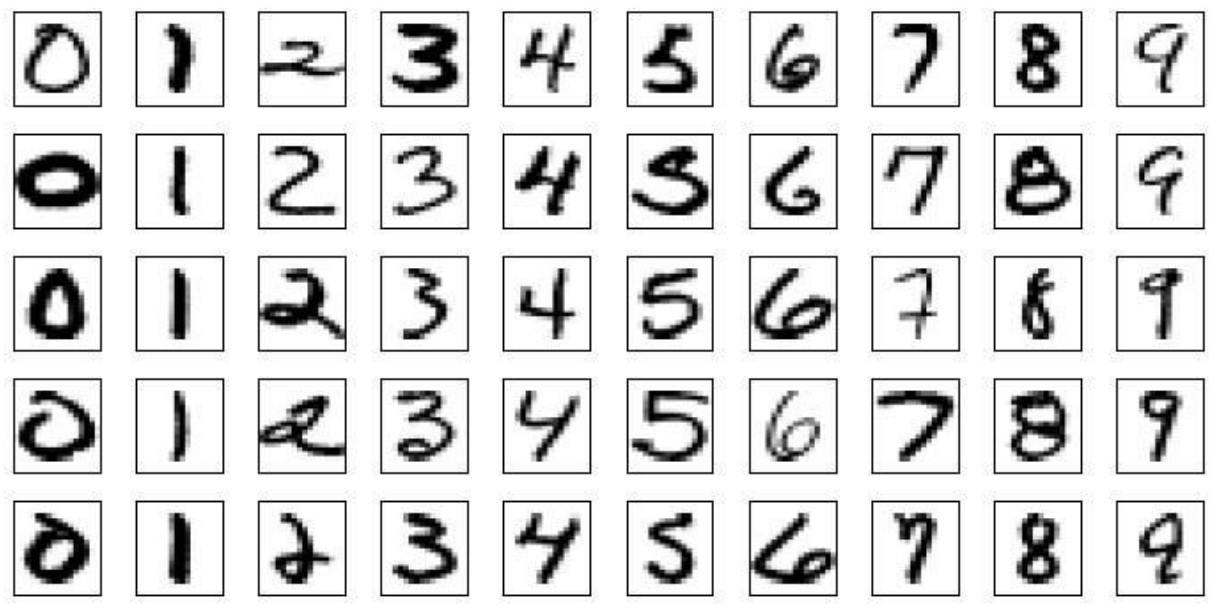
\includegraphics[width=0.69\linewidth,height=0.42\textheight,keepaspectratio]{images/16-cnn_zip.png}
\caption{Esempi dal dataset ZIP code: immagini normalizzate 16×16 a 8 bit in
scala di grigi (Le Cun et al., 1990). Il benchmark MNIST è ``la
drosofila del ML''.}
\end{figure}

Un primo approccio è una rete standard con \textbf{256 input} (uno per
pixel, \(16 \times 16\)): si ottiene un errore del 5--20\%, con molti
errori dovuti alla \textbf{mancanza di invarianza} a rotazioni,
traslazioni, ecc. Una rete completamente connessa tratta ogni pixel come
un input indipendente: non ``sa'' che pixel vicini sono correlati né che
uno stesso tratto può comparire in posizioni diverse.

\begin{boxtip}{L'idea di base}

Sfruttare l'\textbf{architettura} per includere \textbf{conoscenza a
priori} nella rete: - \textbf{connessioni locali} (campi recettivi
locali): ogni unità vede solo una piccola zona dell'immagine, ed estrae
\textbf{feature locali}; - \textbf{condivisione dei pesi} (\emph{weight
sharing}) tra unità diverse: la \textbf{stessa operazione} viene
applicata a parti diverse dell'input, perché le feature di un carattere
possono comparire ovunque nell'immagine (indipendentemente da posizione,
piccole rotazioni\ldots). Si riduce il numero di parametri liberi pur
mantenendo una connettività complessa.

\end{boxtip}

\section{La convoluzione}\label{la-convoluzione}

Il nome viene dall'\textbf{operatore di convoluzione}: una media pesata
di una funzione \(f\), pesata da un'altra funzione \(g\) che scorre nel
tempo: \[
(f * g)(t) = \int_{-\infty}^{\infty} f(\tau)\,g(t - \tau)\,d\tau.
\] L'immagine di \(g\) è limitata (non nulla solo su un intervallo):
\(g\) agisce come una \textbf{finestra scorrevole}.

\subsection{Convoluzione 1D: una unità su uno
stream}\label{convoluzione-1d-una-unituxe0-su-uno-stream}

Un'unità con tre pesi che scorre su una sequenza di input: \[
out_t = \sum_{i=1}^{3} w_i\,x_{t+i-2}.
\]

\begin{figure}[htbp]
\centering
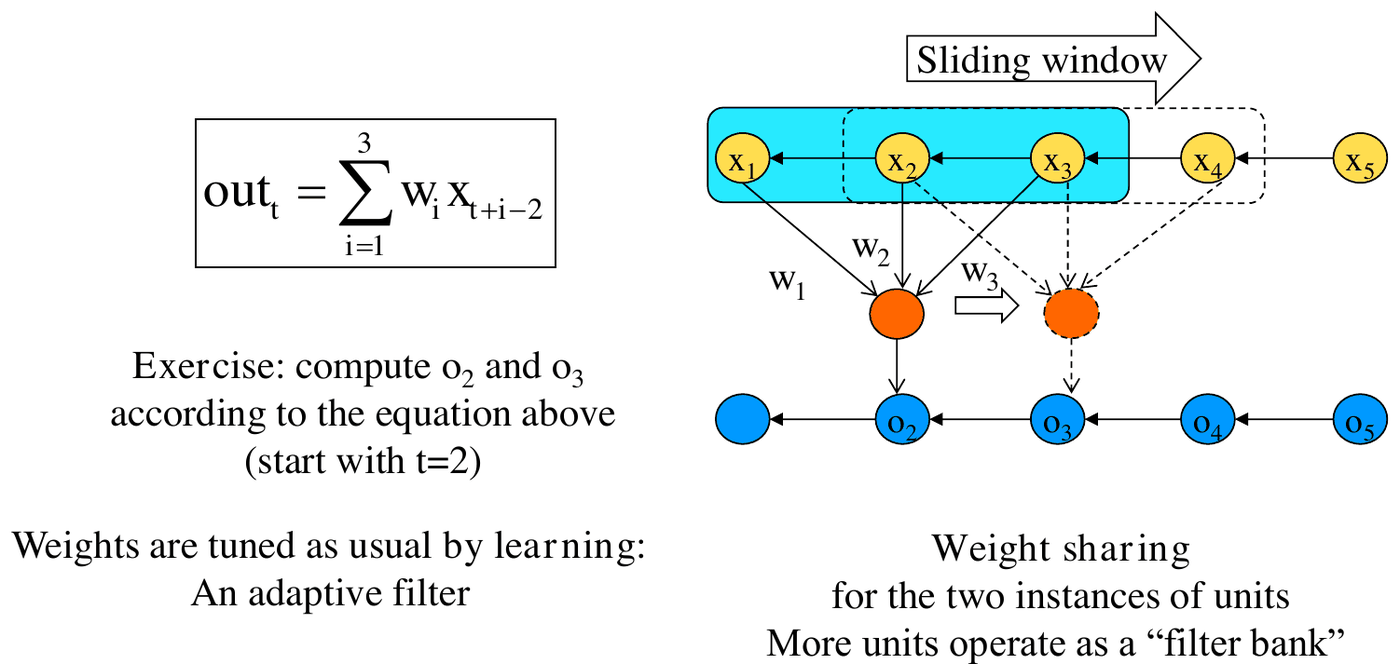
\includegraphics[width=0.80\linewidth,height=0.42\textheight,keepaspectratio]{images/16-cnn_conv1d.png}
\caption{Convoluzione 1D: la stessa unità (con gli stessi pesi) scorre
sull'input.}
\end{figure}

(Esercizio: con \(t = 2\), \(o_2 = w_1x_1 + w_2x_2 + w_3x_3\); con
\(t = 3\), \(o_3 = w_1x_2 + w_2x_3 + w_3x_4\).) I pesi sono
\textbf{condivisi} tra le istanze dell'unità e vengono appresi come al
solito: l'unità è un \textbf{filtro adattivo}. Più unità diverse formano
un \textbf{banco di filtri}. Questa rete si chiama anche
\emph{Time-Delay Neural Network}.

\subsection{Convoluzione 2D}\label{convoluzione-2d}

Su un'immagine si usa un \textbf{kernel} 2D, ad esempio \(3 \times 3\)
(il \textbf{campo recettivo locale} dell'unità), che si sposta di un
pixel alla volta (\textbf{stride} 1). Il \textbf{padding} gestisce i
bordi. Il kernel scorre sull'immagine e produce una \textbf{feature map}
(le feature estratte dal filtro).

In termini di reti neurali: si percorre l'immagine con \textbf{lo stesso
neurone}, che usa connessioni locali.

\begin{figure}[htbp]
\centering
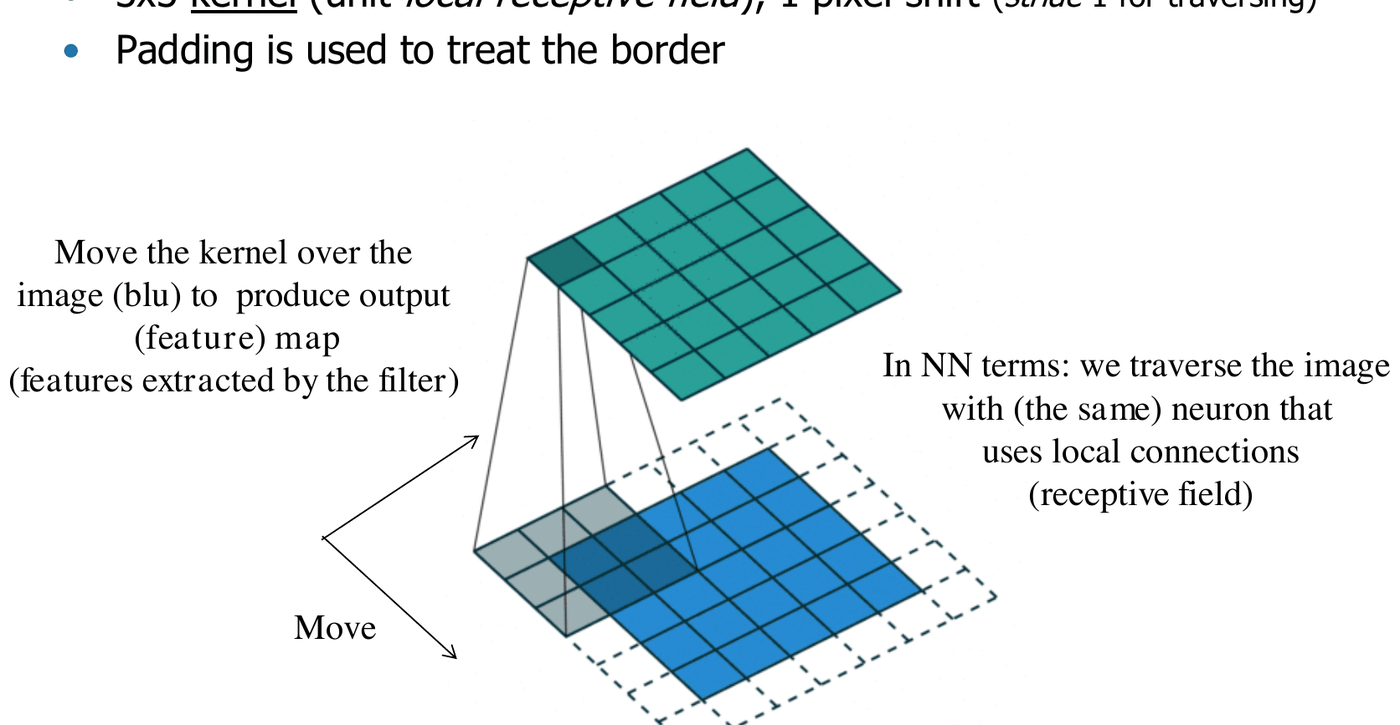
\includegraphics[width=0.80\linewidth,height=0.42\textheight,keepaspectratio]{images/16-cnn_conv2d.png}
\caption{Convoluzione 2D: il kernel scorre sull'immagine e produce la feature
map.}
\end{figure}

\begin{figure}[htbp]
\centering
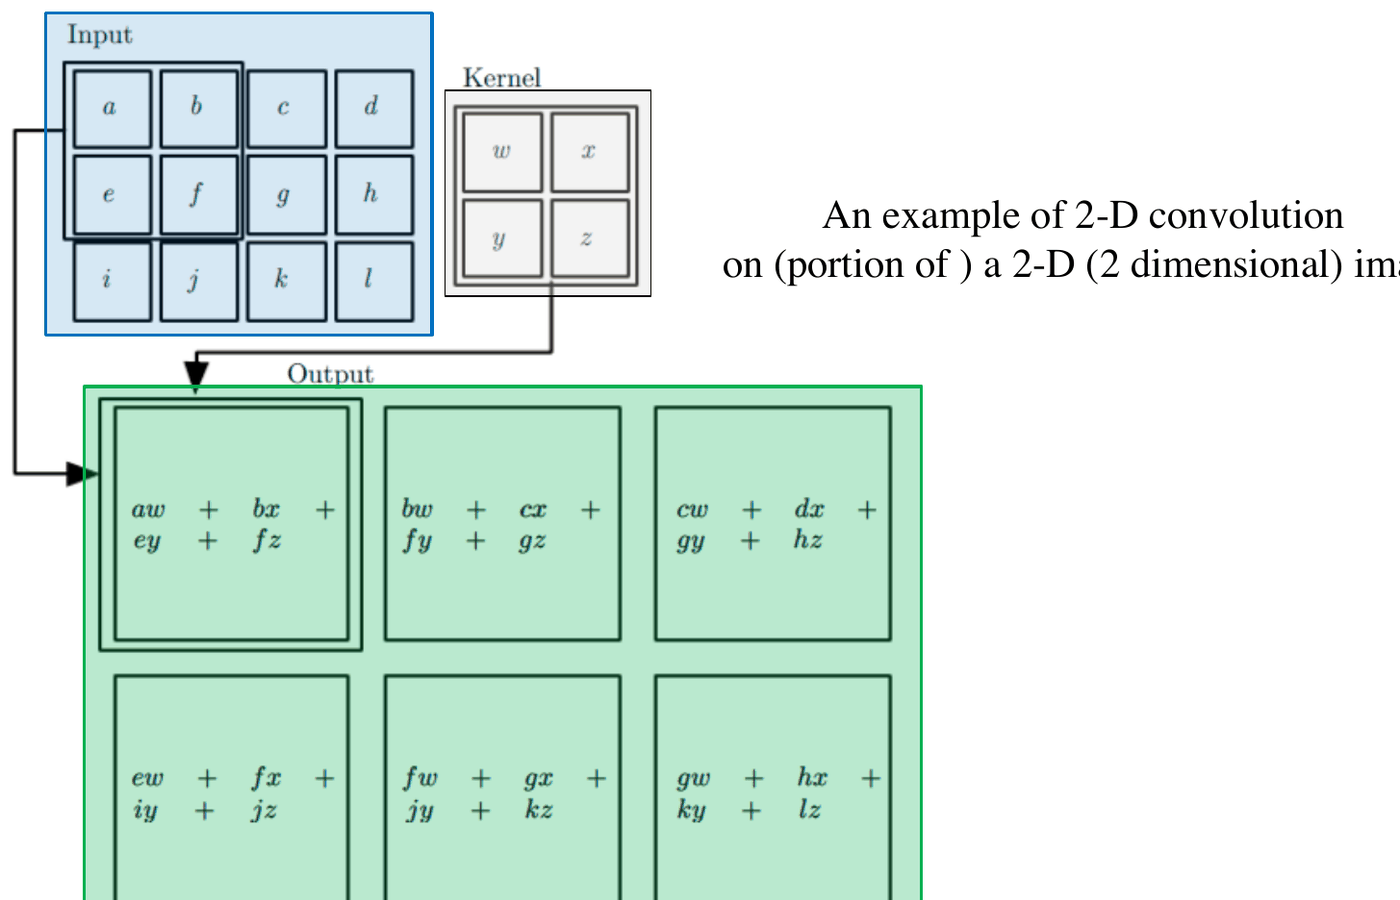
\includegraphics[width=0.66\linewidth,height=0.42\textheight,keepaspectratio]{images/16-cnn_conv2d-esempio.png}
\caption{Esempio di convoluzione 2D di un input 3×4 con un kernel 2×2.}
\end{figure}

\begin{boxnote}{Forma usata nelle librerie}

La convoluzione 2D di un'immagine \(I\) con un kernel \(K\) è
\(S(i,j) = (I * K)(i,j) = \sum_m\sum_n I(m,n)\,K(i-m, j-n)\). Molte
librerie per CNN implementano in realtà la \textbf{cross-correlazione}:
\(S(i,j) = \sum_m\sum_n I(i+m, j+n)\,K(m,n)\) (per i dettagli:
\emph{Deep Learning book}, sez. 9.1; non richiesto all'orale).

\end{boxnote}

\subsection{Stride maggiore di 1}\label{stride-maggiore-di-1}

Con \textbf{stride} \textgreater{} 1 il kernel ``salta'' pixel (ad
esempio due alla volta): è un \textbf{sotto-campionamento}, e produce
una feature map ridotta.

\begin{figure}[htbp]
\centering
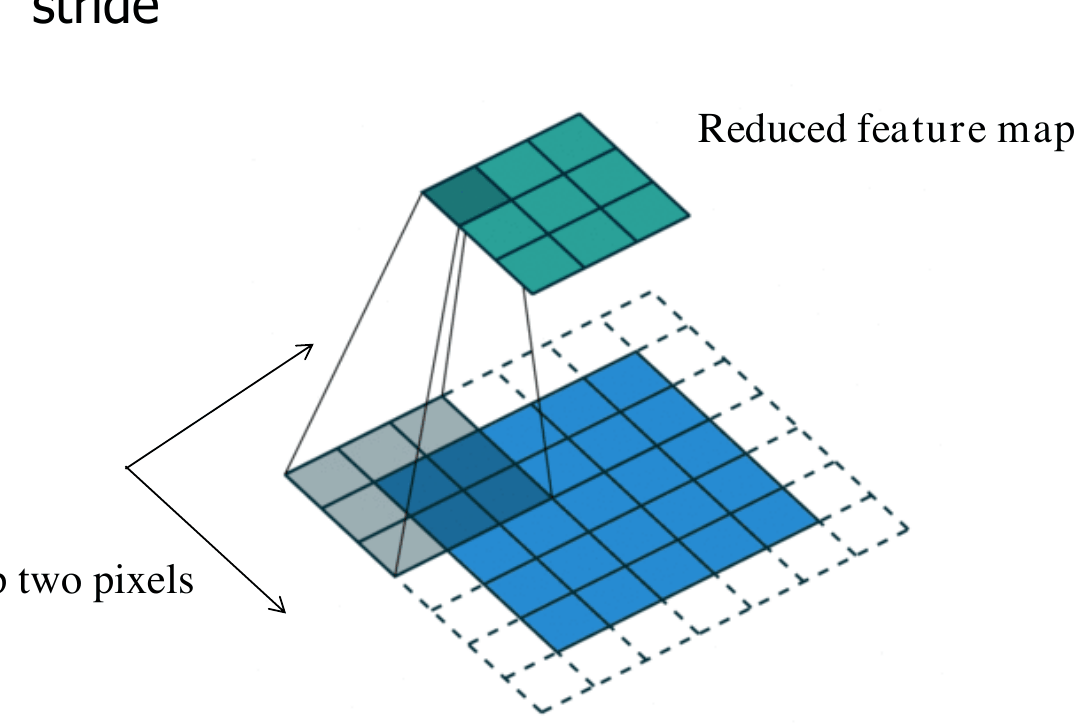
\includegraphics[width=0.51\linewidth,height=0.42\textheight,keepaspectratio]{images/16-cnn_stride.png}
\caption{Convoluzione con stride 2: la feature map risultante è ridotta.}
\end{figure}

\section{Una rete di ``filtri''}\label{una-rete-di-filtri}

I pesi delle unità sono un \textbf{filtro addestrato} a rilevare certe
feature o pattern nell'immagine. Il progetto dell'architettura prevede:

\begin{itemize}
\tightlist
\item
  \textbf{campo recettivo piccolo e locale}: grazie a questo vincolo, i
  filtri appresi rispondono al massimo a pattern \textbf{spazialmente
  locali} (come nella corteccia visiva degli animali);
\item
  \textbf{lo stesso filtro applicato su tutta l'immagine}: le feature
  vengono rilevate \textbf{indipendentemente dalla posizione}, ottenendo
  l'\textbf{invarianza per traslazione};
\item
  \textbf{filtri appresi}: i filtri che negli algoritmi tradizionali di
  elaborazione di immagini erano progettati a mano vengono
  \textbf{appresi}. L'indipendenza dalla conoscenza a priori e dallo
  sforzo umano nel progettare le feature è un grande vantaggio;
\item
  \textbf{molti strati impilati}: le unità delle feature map
  rappresentano aree via via più grandi dell'immagine originale
  (assemblando aree delle mappe precedenti).
\end{itemize}

\section{Pooling}\label{pooling}

Il \textbf{pooling} riduce la feature map:

\begin{itemize}
\tightlist
\item
  con sotto-campionamento (stride \textgreater{} 1, visto sopra);
\item
  con una \textbf{media} (semplice o pesata);
\item
  con il \textbf{max pooling} (il più comune).
\end{itemize}

In pratica, invece di produrre un valore per ogni pixel di input, se ne
produce uno per un insieme (rettangolare) di pixel, prendendo la media o
il massimo delle uscite.

\begin{figure}[htbp]
\centering
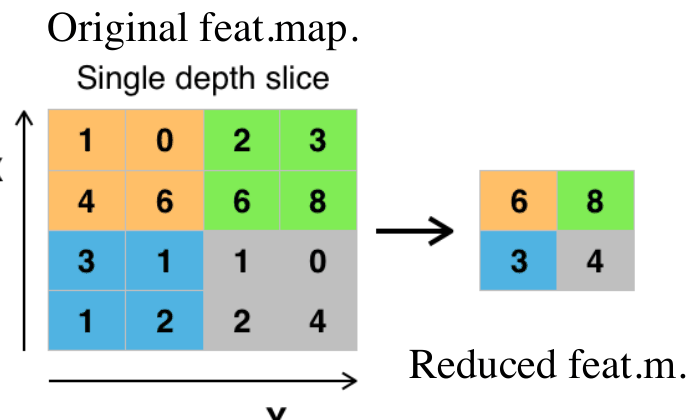
\includegraphics[width=0.40\linewidth,height=0.42\textheight,keepaspectratio]{images/16-cnn_maxpool.png}
\caption{Max pooling con filtro 2×2 e stride 2.}
\end{figure}

Il pooling aiuta anche a rendere la rappresentazione
\textbf{approssimativamente invariante a piccole traslazioni}
dell'input: il massimo (o la media) cambia poco se l'input si sposta di
poco, quindi un'uscita alta resta alta per una versione leggermente
traslata.

\section{La CNN nel complesso}\label{la-cnn-nel-complesso}

Una CNN sfrutta la condivisione dei pesi per realizzare una finestra
scorrevole di campi locali su un segnale, estesa alle immagini 2D e
ripetuta su molti strati (feature map), alternata a operazioni di
pooling. I quattro ingredienti:

\begin{enumerate}
\def\labelenumi{\arabic{enumi}.}
\tightlist
\item
  \textbf{connessioni locali};
\item
  \textbf{pesi condivisi};
\item
  \textbf{pooling};
\item
  \textbf{molti strati}.
\end{enumerate}

\begin{figure}[htbp]
\centering
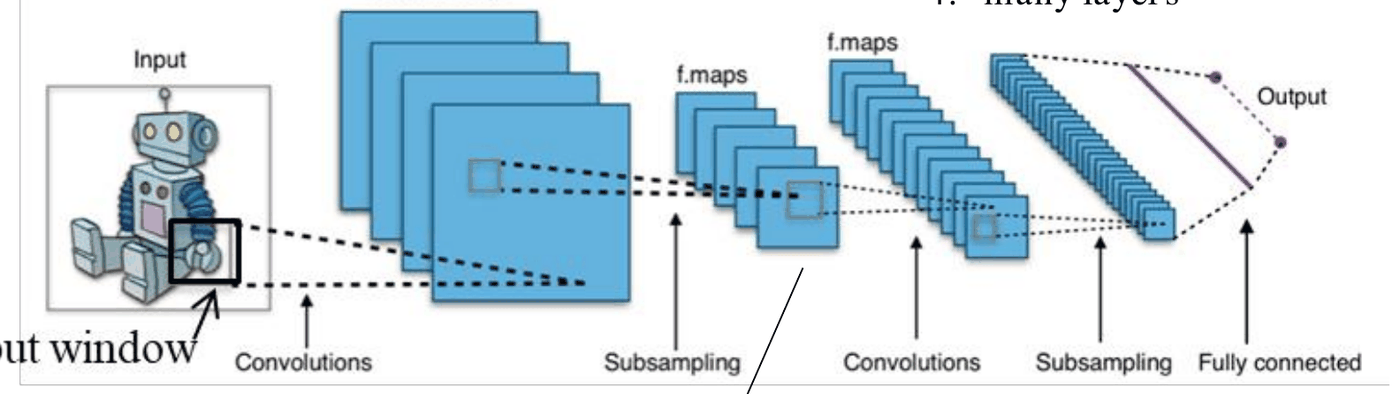
\includegraphics[width=0.89\linewidth,height=0.42\textheight,keepaspectratio]{images/16-cnn_cnn-intera.png}
\caption{Una CNN completa: convoluzioni e sotto-campionamenti alternati, seguiti
da strati completamente connessi. Il numero di filtri (feature map) può
crescere negli strati più alti.}
\end{figure}

\begin{figure}[htbp]
\centering
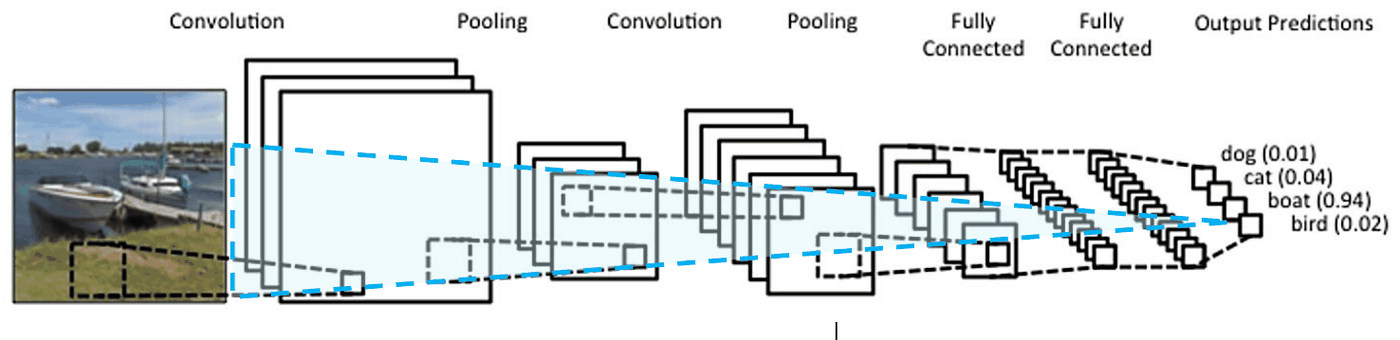
\includegraphics[width=0.89\linewidth,height=0.42\textheight,keepaspectratio]{images/16-cnn_esempio2.png}
\caption{Il ``cono'' dall'immagine alle mappe finali: il campo recettivo delle
unità finali è molto più ampio di quello delle unità dei primi strati,
perché sono collegate indirettamente a gran parte dell'immagine.}
\end{figure}

\begin{figure}[htbp]
\centering
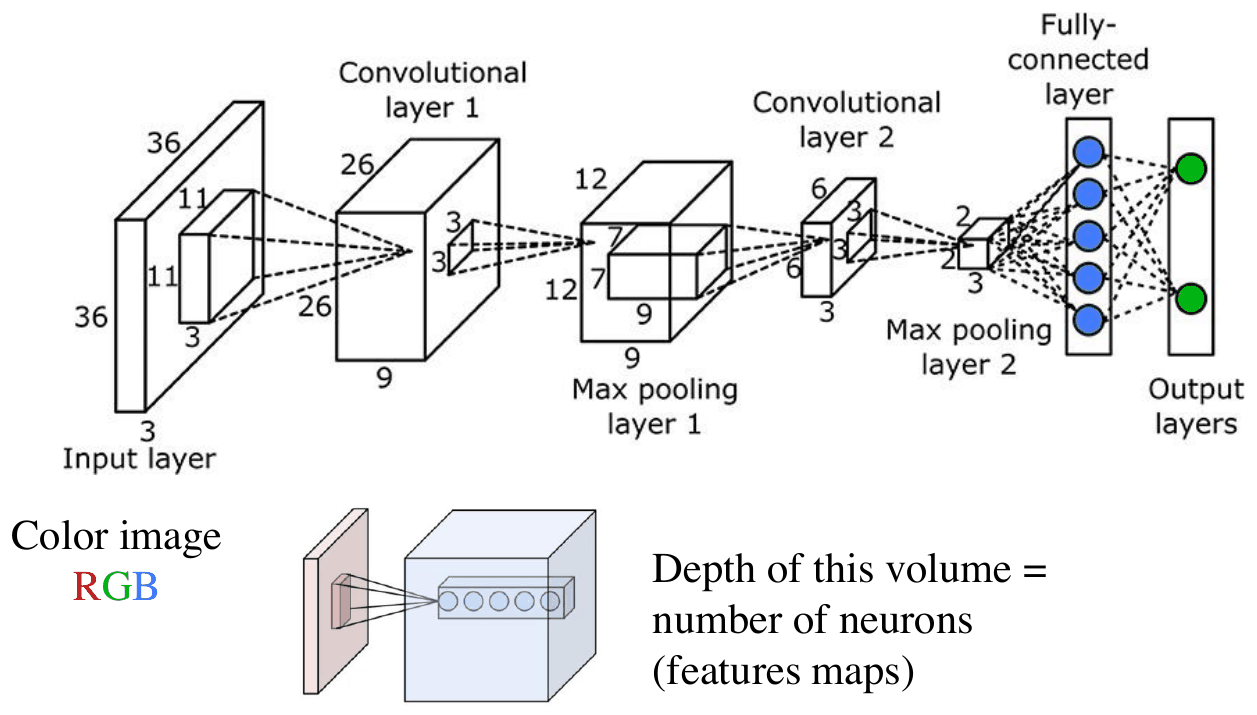
\includegraphics[width=0.71\linewidth,height=0.42\textheight,keepaspectratio]{images/16-cnn_esempio3.png}
\caption{Un esempio con le dimensioni; per un'immagine a colori (RGB) la
profondità del volume è il numero di feature map.}
\end{figure}

\begin{figure}[htbp]
\centering
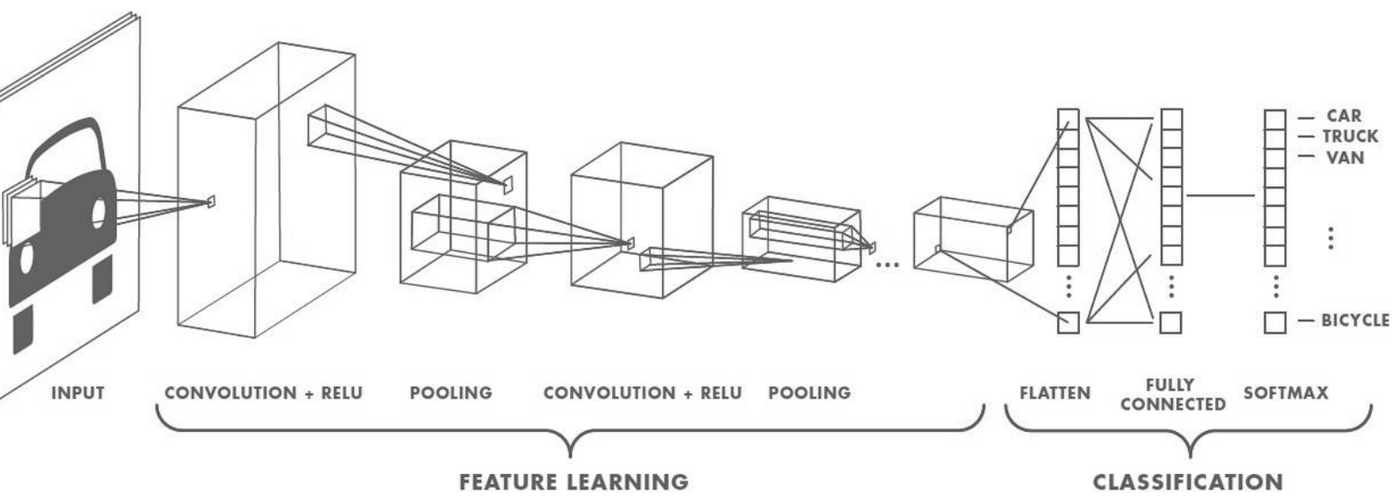
\includegraphics[width=0.89\linewidth,height=0.42\textheight,keepaspectratio]{images/16-cnn_alexnet.png}
\caption{Un'architettura tipo AlexNet: una parte di}
\end{figure}

\begin{boxabstract}{Vantaggi delle CNN}

\begin{itemize}
\tightlist
\item
  \textbf{Connessioni locali e pesi condivisi}: rilevano motivi/pattern
  locali nelle immagini, in modo \textbf{invariante alla traslazione}
  (alla posizione del pattern); \textbf{riducono il numero di parametri
  liberi} pur mantenendo le connessioni, il che è una forma di
  \textbf{regolarizzazione}.
\item
  \textbf{Pooling}: riduce la dimensione della rappresentazione a ogni
  strato (una \textbf{piramide} di strati) e aiuta l'invarianza a
  piccoli spostamenti e distorsioni.
\item
  \textbf{Molti strati}: le operazioni 1 e 2 applicate a tutte le
  feature map producono un'\textbf{astrazione progressiva} delle
  feature, permettendo di \textbf{comporre primitive} (feature di basso
  livello, apprese una volta sola) in tutte le combinazioni possibili
  negli strati successivi.
\item
  Sono un'istanza storica di \textbf{rete profonda}, e sono state
  studiate analogie con il sistema visivo (neuroscienze).
\end{itemize}

\end{boxabstract}

\section{Come si usano}\label{come-si-usano}

L'addestramento avviene tipicamente con la \textbf{backpropagation}, con
le euristiche note e alcune specializzazioni (per la condivisione dei
pesi, il pooling\ldots). Visto l'uso tipico di reti enormi e grandi
quantità di dati, molti iperparametri vengono fissati \textbf{per
esperienza} o su suggerimento di esperti, perché sarebbe troppo costoso
fare cross-validation su grandi spazi di iperparametri. Addestramento,
effetti di regolarizzazione e buon comportamento di queste reti enormi
saranno discussi nel quadro del deep learning.

\section{Risultati storici}\label{risultati-storici}

\subsection{Le architetture di LeCun sul dataset ZIP
code}\label{le-architetture-di-lecun-sul-dataset-zip-code}

\begin{figure}[htbp]
\centering
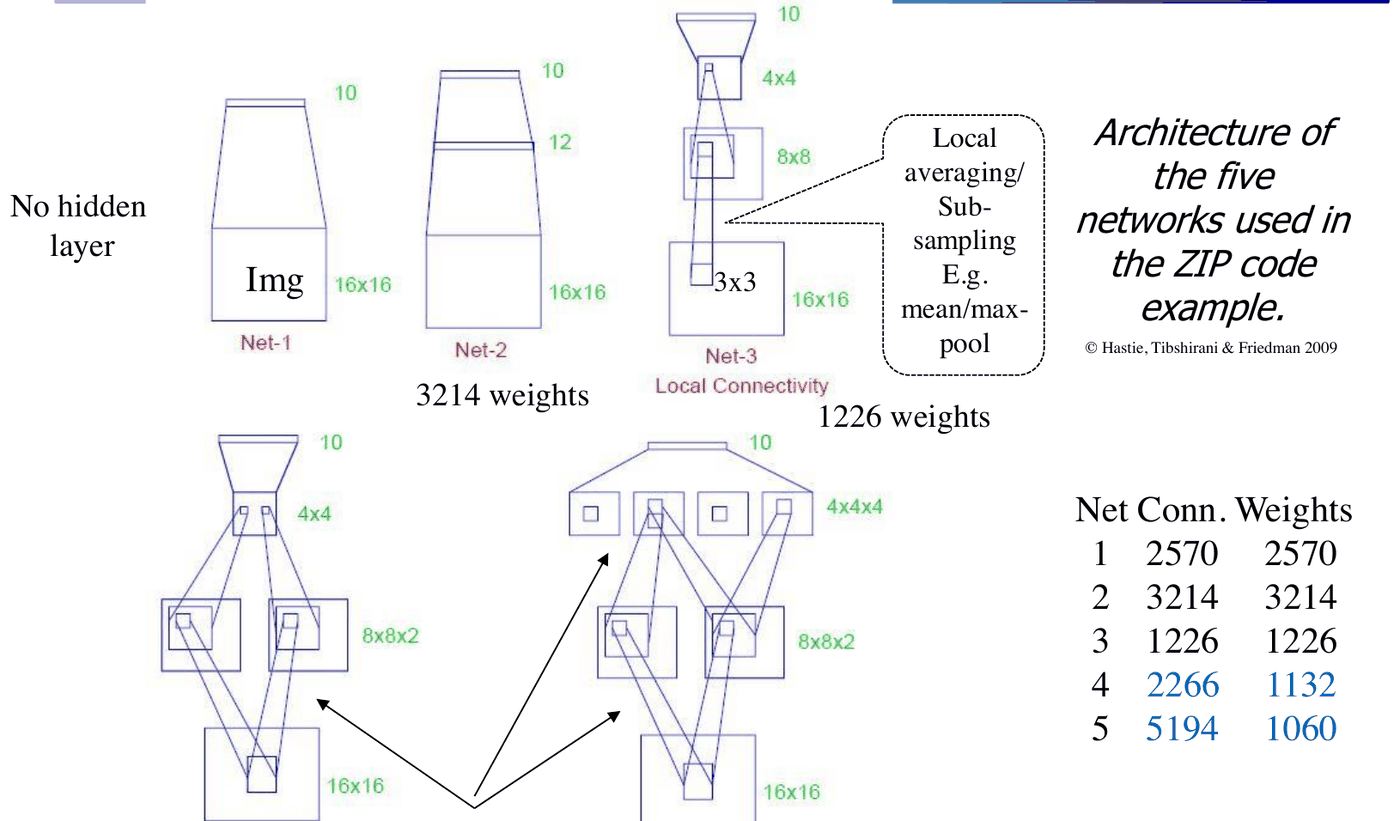
\includegraphics[width=0.89\linewidth,height=0.42\textheight,keepaspectratio]{images/16-cnn_lecun.png}
\caption{Le cinque reti usate da LeCun sul problema ZIP code: da una rete senza
strati nascosti (Net-1) a reti con connessioni locali (Net-3) e pesi
condivisi (Net-4, Net-5).}
\end{figure}

{\def\LTcaptype{none} % do not increment counter
\begin{longtable}[]{@{}lll@{}}
\toprule\noalign{}
Rete & Connessioni & Pesi \\
\midrule\noalign{}
\endhead
\bottomrule\noalign{}
\endlastfoot
Net-1 & 2570 & 2570 \\
Net-2 & 3214 & 3214 \\
Net-3 & 1226 & 1226 \\
Net-4 & 2266 & 1132 \\
Net-5 & 5194 & 1060 \\
\end{longtable}
}

Con i pesi condivisi il numero di \textbf{connessioni} può crescere
mentre il numero di \textbf{pesi} (parametri liberi) resta basso.

\begin{figure}[htbp]
\centering
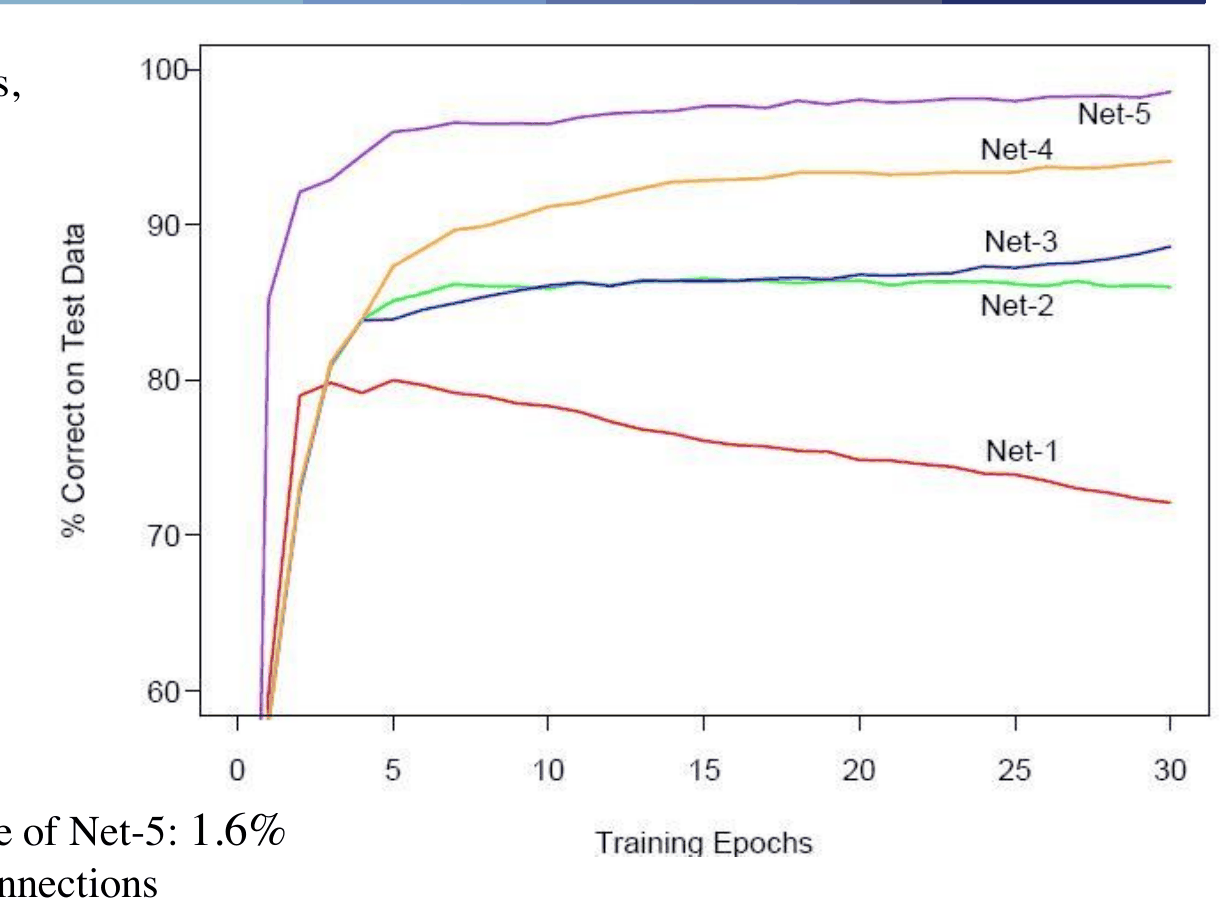
\includegraphics[width=0.63\linewidth,height=0.42\textheight,keepaspectratio]{images/16-cnn_lecun-curve.png}
\caption{Curve di prestazione sul test per le cinque reti (Le Cun, 1989).
L'errore di training è zero per tutte, su un insieme ridotto di circa
300 immagini.}
\end{figure}

Net-5 raggiunge un errore dell'\textbf{1,6\%} con 5194 connessioni e
soli 1060 pesi. Oggi si arriva allo 0,8\% (con reti e SVM) e anche meno.

\subsection{MNIST}\label{mnist}

Il dataset completo ha 60.000 immagini di training e 10.000 di test. I
progressi (1998--2012) sono documentati sul sito di LeCun. Con il deep
learning (MLP o CNN con molti strati, pre-addestramento non
supervisionato strato per strato) si è arrivati allo 0,39\% (2006) e
0,35\% (2011); il migliore nel 2012 è lo 0,23\% (comitato di reti
convoluzionali), 0,21\% nel 2016.

\begin{boxwarning}{Attenzione}

Il test set di MNIST è stato usato così tante volte che i miglioramenti
dell'ordine dello 0,1\% non sono più significativi: è di fatto diventato
un validation set per la comunità.

\end{boxwarning}

\begin{boxnote}{Anche un MLP profondo funziona?}

Un articolo del 2010 (\emph{Neural Computation}) mostra che la ``buona
vecchia'' backpropagation on-line su un semplice MLP ottiene lo 0,35\%
su MNIST: bastano \textbf{molti strati}, \textbf{molti neuroni} per
strato, \textbf{molte immagini deformate} per il training e \textbf{GPU}
per accelerare. La rete 784-2500-2000-1500-1000-500-10 ha 12 milioni di
pesi e si addestra in 2 ore. Il controllo della complessità è ottenuto
deformando le immagini per avere molti più esempi (\emph{data
augmentation}).

\end{boxnote}

\subsection{Riconoscimento facciale e
ImageNet}\label{riconoscimento-facciale-e-imagenet}

\begin{itemize}
\tightlist
\item
  \textbf{DeepFace} (CVPR 2014): reti convoluzionali a 9 strati
  addestrate su 4 milioni di immagini di più di 4000 persone; riconosce
  se due foto mostrano la stessa persona con accuratezza del 97,25\%
  (umani: 97,53\%).
\item
  \textbf{AlexNet} (Krizhevsky, Sutskever, Hinton, NIPS 2012): una CNN
  profonda addestrata su 1,3 milioni di immagini ad alta risoluzione di
  ImageNet (ILSVRC-2010) in 1000 classi. Errori top-1 e top-5 del 39,7\%
  e 18,9\% (dal precedente \textasciitilde26\%), molto meglio dello
  stato dell'arte. La rete ha \textbf{60 milioni di parametri} e 500.000
  neuroni: cinque strati convoluzionali (alcuni seguiti da max pooling)
  e due strati completamente connessi con softmax finale a 1000 classi.
  Per velocizzare l'addestramento: neuroni \textbf{non saturanti} (ReLU)
  e un'implementazione GPU molto efficiente. Per ridurre l'overfitting
  negli strati densi: un nuovo metodo di regolarizzazione, il
  \textbf{dropout}.
\end{itemize}

\begin{figure}[htbp]
\centering
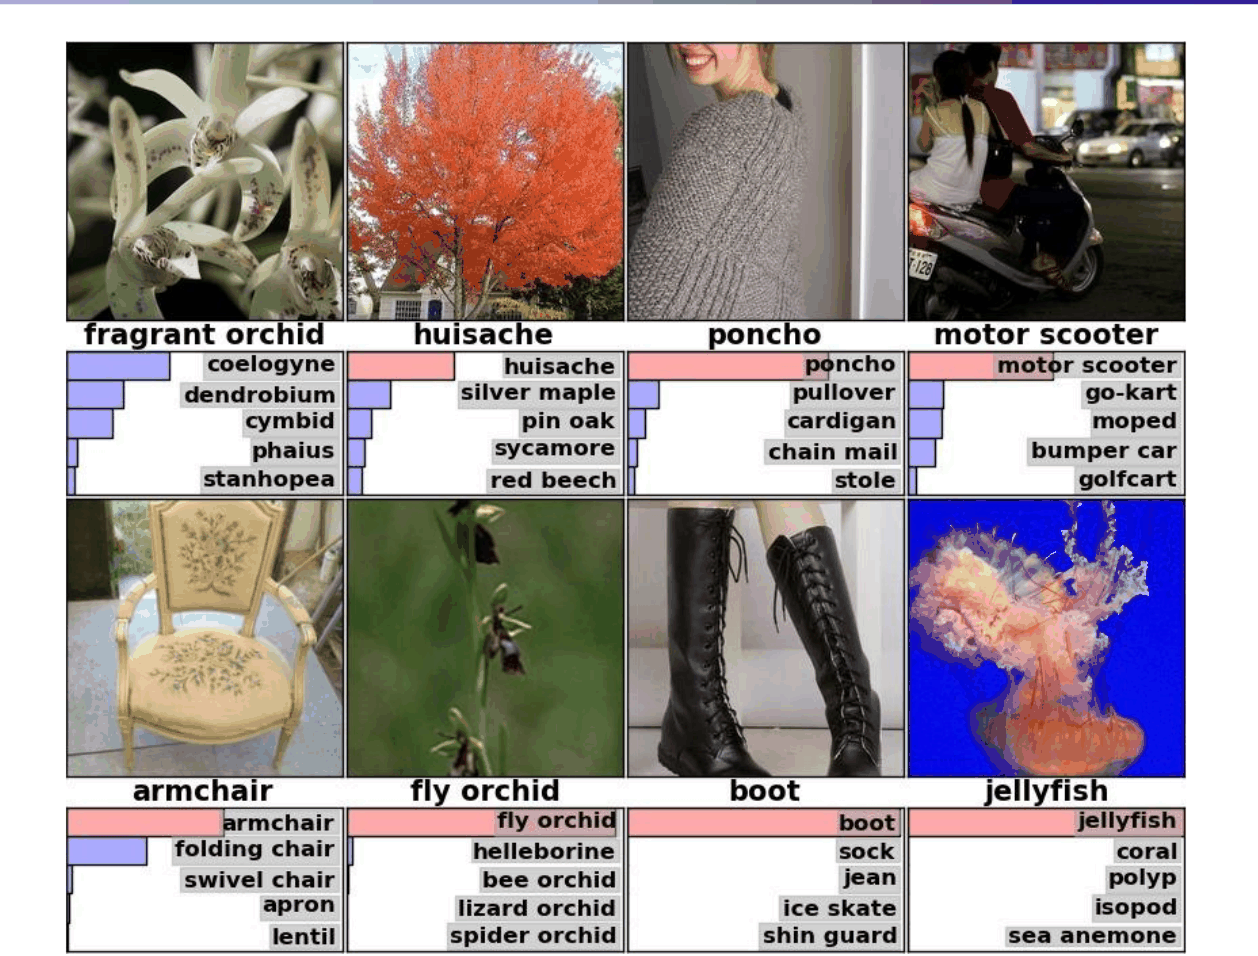
\includegraphics[width=0.63\linewidth,height=0.42\textheight,keepaspectratio]{images/16-cnn_imagenet.png}
\caption{Predizioni top-5 di AlexNet su immagini casuali del test set.}
\end{figure}

\section{CNN moderne e GPU}\label{cnn-moderne-e-gpu}

Esistono molte varianti e architetture specializzate per le immagini
(corso \emph{Intelligent Systems for Pattern Recognition}), con grande
impatto su Pattern Recognition e Computer Vision; le basi
neuroscientifiche sono trattate nel corso di \emph{Computational
Neuroscience}. Si possono anche riusare le feature di modelli
\textbf{già addestrati} su grandi benchmark (AlexNet, GoogLeNet, VGG,
ResNet\ldots): sono disponibili molte CNN pre-addestrate per
classificazione, segmentazione, riconoscimento facciale, rilevamento di
testo.

Le implementazioni efficienti sfruttano le \textbf{GPU} tramite la
rappresentazione a \textbf{tensori}. La moltiplicazione di matrici (cioè
i prodotti scalari) è un'operazione lineare che le GPU eseguono in modo
molto efficiente, parallelizzando le somme e i prodotti indipendenti.
Molte operazioni di kernel si possono scrivere come un'unica
moltiplicazione tra matrici a blocchi; la notazione a \textbf{tensori}
(array multidimensionali con l'operazione \emph{tensordot}, ad esempio
in TensorFlow o NumPy) permette di farlo senza costruire a mano matrici
a blocchi complesse.

\begin{boxnote}{Oltre le CNN: le Capsule Network}

Le \textbf{Capsule Network} (Sabour, Frosst, Hinton, 2017) usano
sotto-reti specializzate: una ``capsula'' è un gruppo di neuroni che
produce sia un parametro che indica se un'entità è presente, sia un
vettore di \textbf{parametri di posa} (posizione, orientamento) rispetto
a una versione canonica. Al posto del max pooling usano un meccanismo di
\textbf{routing} (l'idea che il cervello instradi l'informazione visiva
di basso livello verso la capsula più adatta). Ottengono ottimi
risultati su MNIST, riconoscendo molto meglio di una CNN cifre
sovrapposte.

\end{boxnote}

\begin{boxquestion}{Possibili domande d'esame}

\begin{itemize}
\tightlist
\item
  Quali sono le idee chiave delle CNN (connessioni locali, pesi
  condivisi, pooling, molti strati) e cosa comporta ciascuna?
\item
  Cos'è la convoluzione in una rete neurale? Cosa sono kernel, stride,
  padding, feature map?
\item
  A cosa serve il pooling? Come funziona il max pooling?
\item
  Perché la condivisione dei pesi è una forma di regolarizzazione?
\item
  Come cresce il campo recettivo con la profondità?
\end{itemize}

\end{boxquestion}
